% anhang.tex
\chapter{Appendix}
\label{chapter:appendix}
\section{Isolated Testing of Memory Bandwidth}
\label{section:stridedmembwtest}
\begin{figure}[h]
  \begin{algorithm}{Loop with Strided Memory Access}{stridedmemoryaccess}
    \begin{lstlisting}[language=C++,basicstyle=\scriptsize\ttfamily,showstringspaces=false]
// Uses 8 strides spaced out 4 KB
for (int iter = 0; iter < NUM_ITERATIONS; iter++) {
  for (size_t i = 0; i < VEC_SIZE - TOTAL_STRIDE_DIST + 1;
       i += TOTAL_STRIDE_DIST) {
    #pragma GCC unroll 1 // prevent loop unrolling
    for (size_t j = i; j < STRIDE_LENGTH + i; j += 8) {
      asm volatile(                        //
          "vmovaps (%0),       %%ymm0\n\t" //
          "vmovaps 0x1000(%0), %%ymm1\n\t" // offset 1 * 4096 bytes
          "vmovaps 0x2000(%0), %%ymm2\n\t" // offset 2 * 4096 bytes
          "vmovaps 0x3000(%0), %%ymm3\n\t" // offset 3 * 4096 bytes
          "vmovaps 0x4000(%0), %%ymm4\n\t" // offset 4 * 4096 bytes
          "vmovaps 0x5000(%0), %%ymm5\n\t" // offset 5 * 4096 bytes
          "vmovaps 0x6000(%0), %%ymm6\n\t" // offset 6 * 4096 bytes
          "vmovaps 0x7000(%0), %%ymm7"     // offset 7 * 4096 bytes
          :
          : "r"(&array[j])                  //
          : "ymm0", "ymm1", "ymm2", "ymm3", //
            "ymm4", "ymm5", "ymm6", "ymm7");
    }
  }
} // Uses sequential memory access
for (int iter = 0; iter < NUM_ITERATIONS; iter++) {
  #pragma GCC unroll 1 // prevent loop unrolling
  for (size_t i = 0; i < VEC_SIZE - 63; i += 64) {
    asm volatile(                      //
        "vmovaps (%0),     %%ymm0\n\t" //
        "vmovaps 0x20(%0), %%ymm1\n\t" // offset 32 bytes <=> 1 AVX2 vector
        "vmovaps 0x40(%0), %%ymm2\n\t" // offset 64 bytes
        "vmovaps 0x60(%0), %%ymm3\n\t" // ...
        "vmovaps 0x80(%0), %%ymm4\n\t"
        "vmovaps 0xa0(%0), %%ymm5\n\t"
        "vmovaps 0xc0(%0), %%ymm6\n\t"
        "vmovaps 0xe0(%0), %%ymm7"
        :
        : "r"(&array[i])                  //
        : "ymm0", "ymm1", "ymm2", "ymm3", //
          "ymm4", "ymm5", "ymm6", "ymm7");
  }
}
    \end{lstlisting}
  \end{algorithm}
\end{figure}
\noindent A C program to test the bandwidth of strided against non-strided memory access was created to isolate "the problem" from other variables. In \autoref{alg:stridedmemoryaccess} are the two loops used in the methods testing the memory read bandwidth. The loops iterate 16 times over a 12 GB array. These are the results from two different machines:
\\\texttt{
  Results from Machine used in previous experiments:\\
  SIMD Read Bandwidth (Sequential)\ \ \ \ \ \ \ \ \ \ \ : 29.46 GB/s\\
  SIMD Read Bandwidth with stride length 4096: 36.71 GB/s\\
  AMD 4800U 8C/16T, 16 GB LPDDR4 2666MHz:\\
  SIMD Read Bandwidth (Sequential)\ \ \ \ \ \ \ \ \ \ \ : 16.39 GB/s\\
  SIMD Read Bandwidth with stride length 4096: 22.74 GB/s\\
}
The results line up very closely with the bandwidth results obtained from the vector similarity search program. But I have no Intel PC at my disposal to test this on a different architecture.

\section{Trying out the Similarity Search Implementation}
\label{sec:tryingout}
Go to \url{https://github.com/thubn/simsearch} for more information. In the main README go to the "Embedding Search Server" link in the index.

\section{Additional Plots}
\begin{figure}[h]
  \makebox[\textwidth][c]{%
    \begin{minipage}{0.49\widefigwidth}
      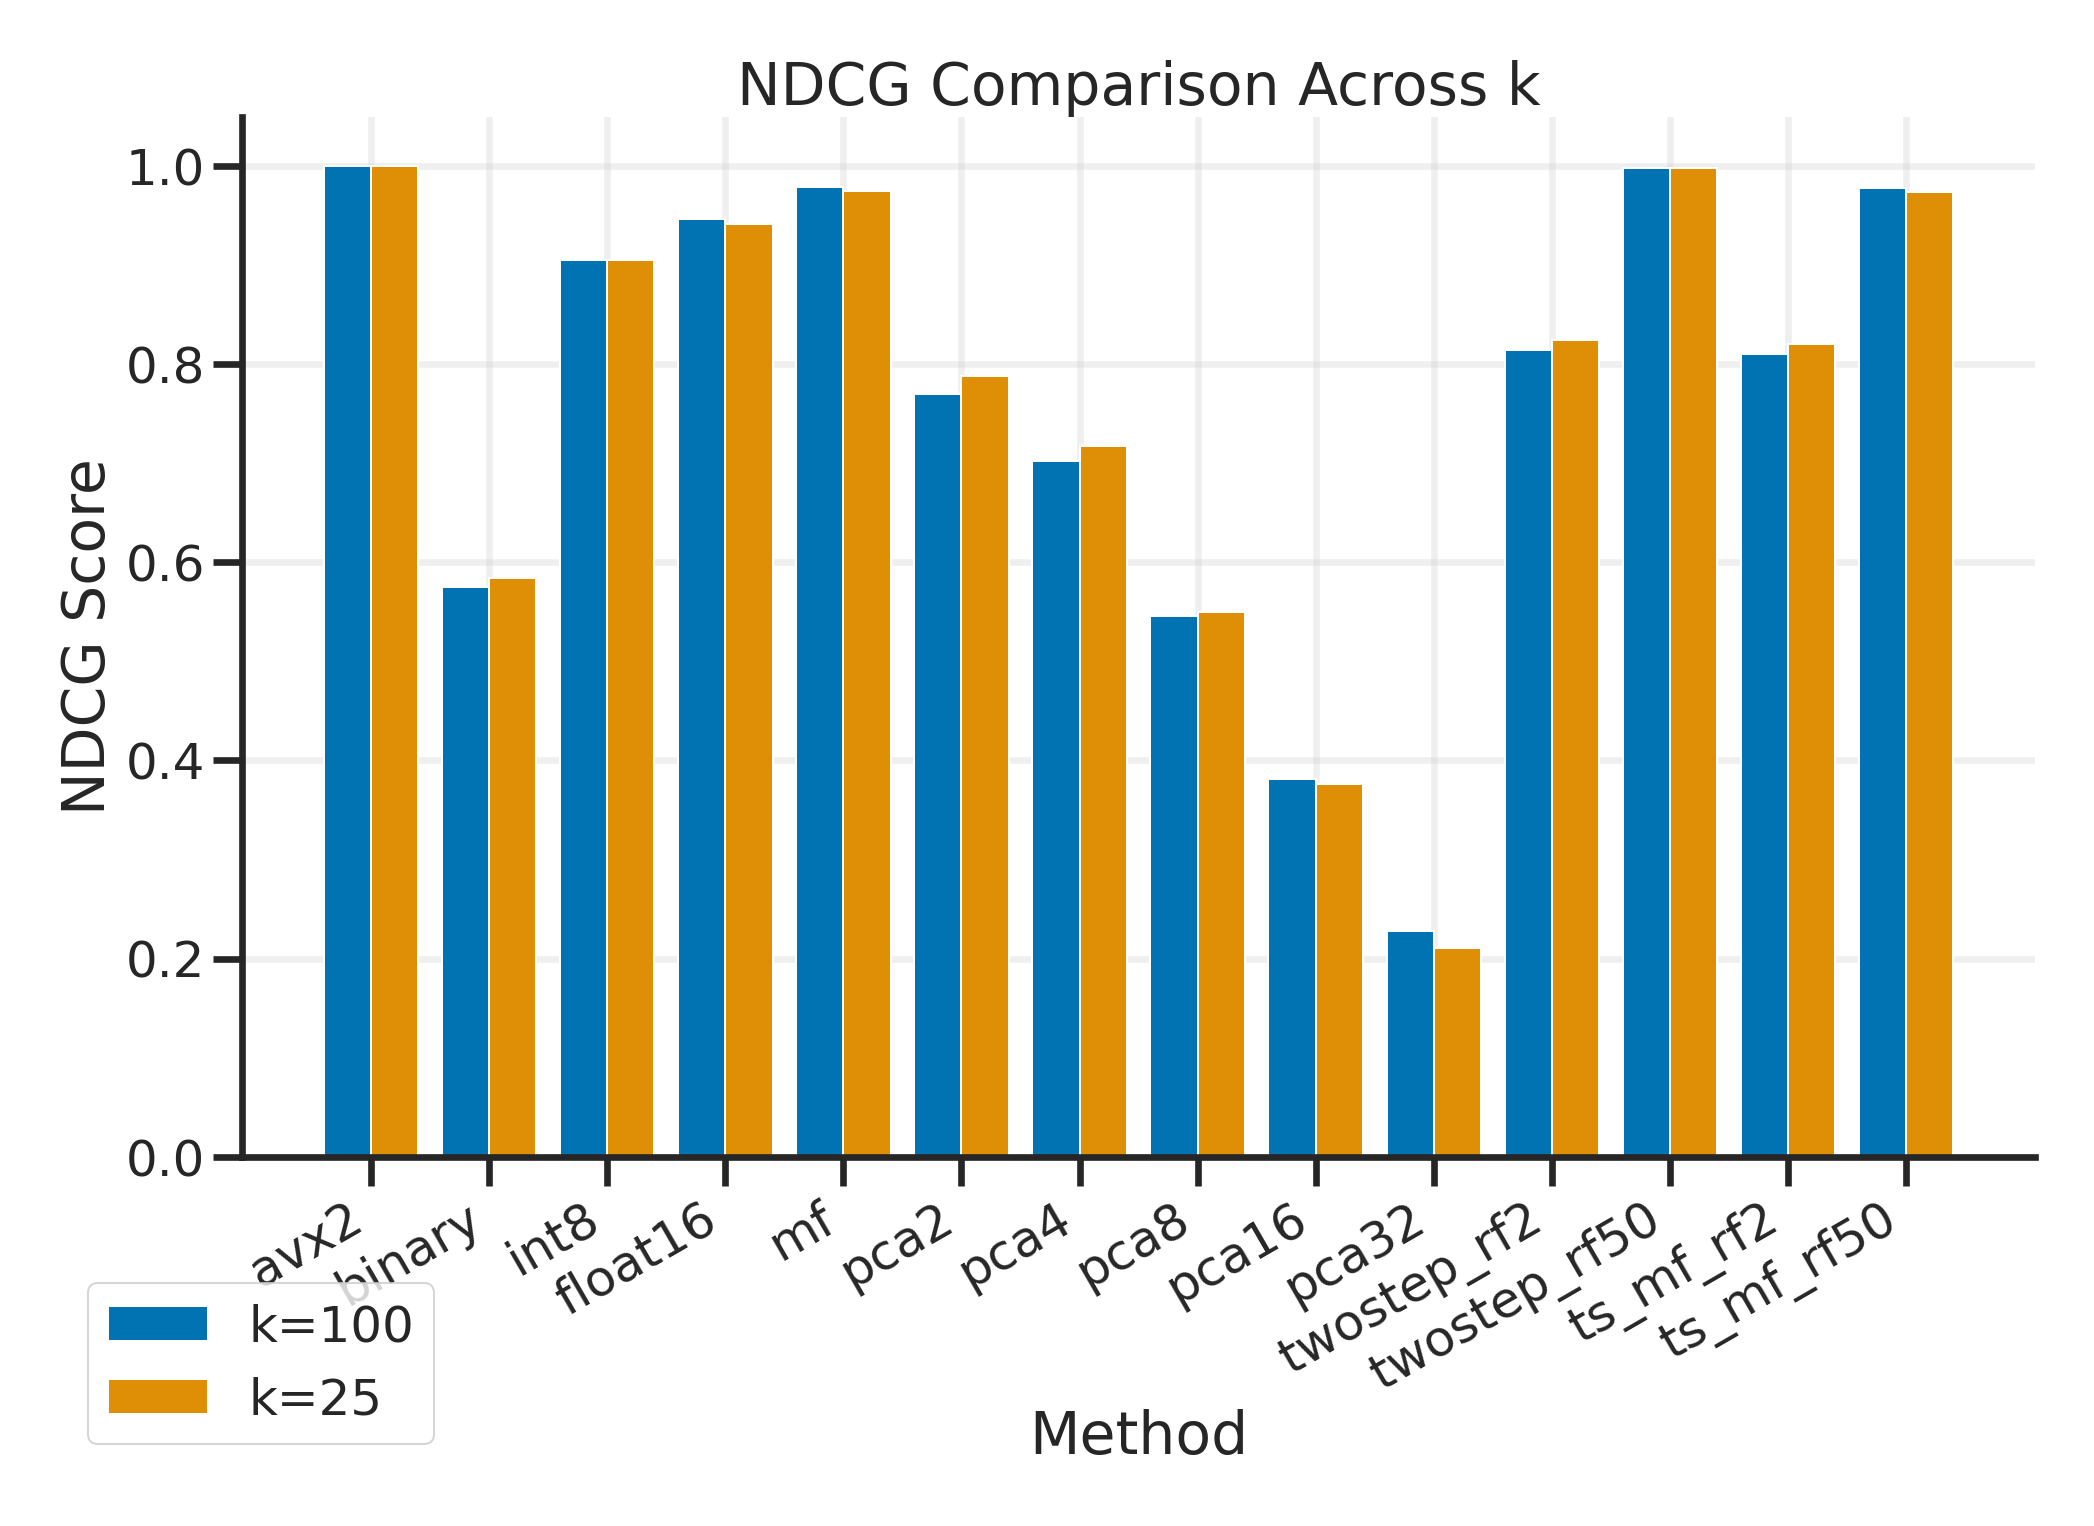
\includegraphics[width=0.49\widefigwidth]{bilder/plots/benchmark_comparison_dim1024_k100_q_dim1024_k25_q_cmp_k.png}
      \vspace{-1cm}
      \caption{Comparing the retrieval accuracy across different k values}
      \label{kcomparison}
    \end{minipage}
    %\hfill
    \begin{minipage}{0.49\widefigwidth}
      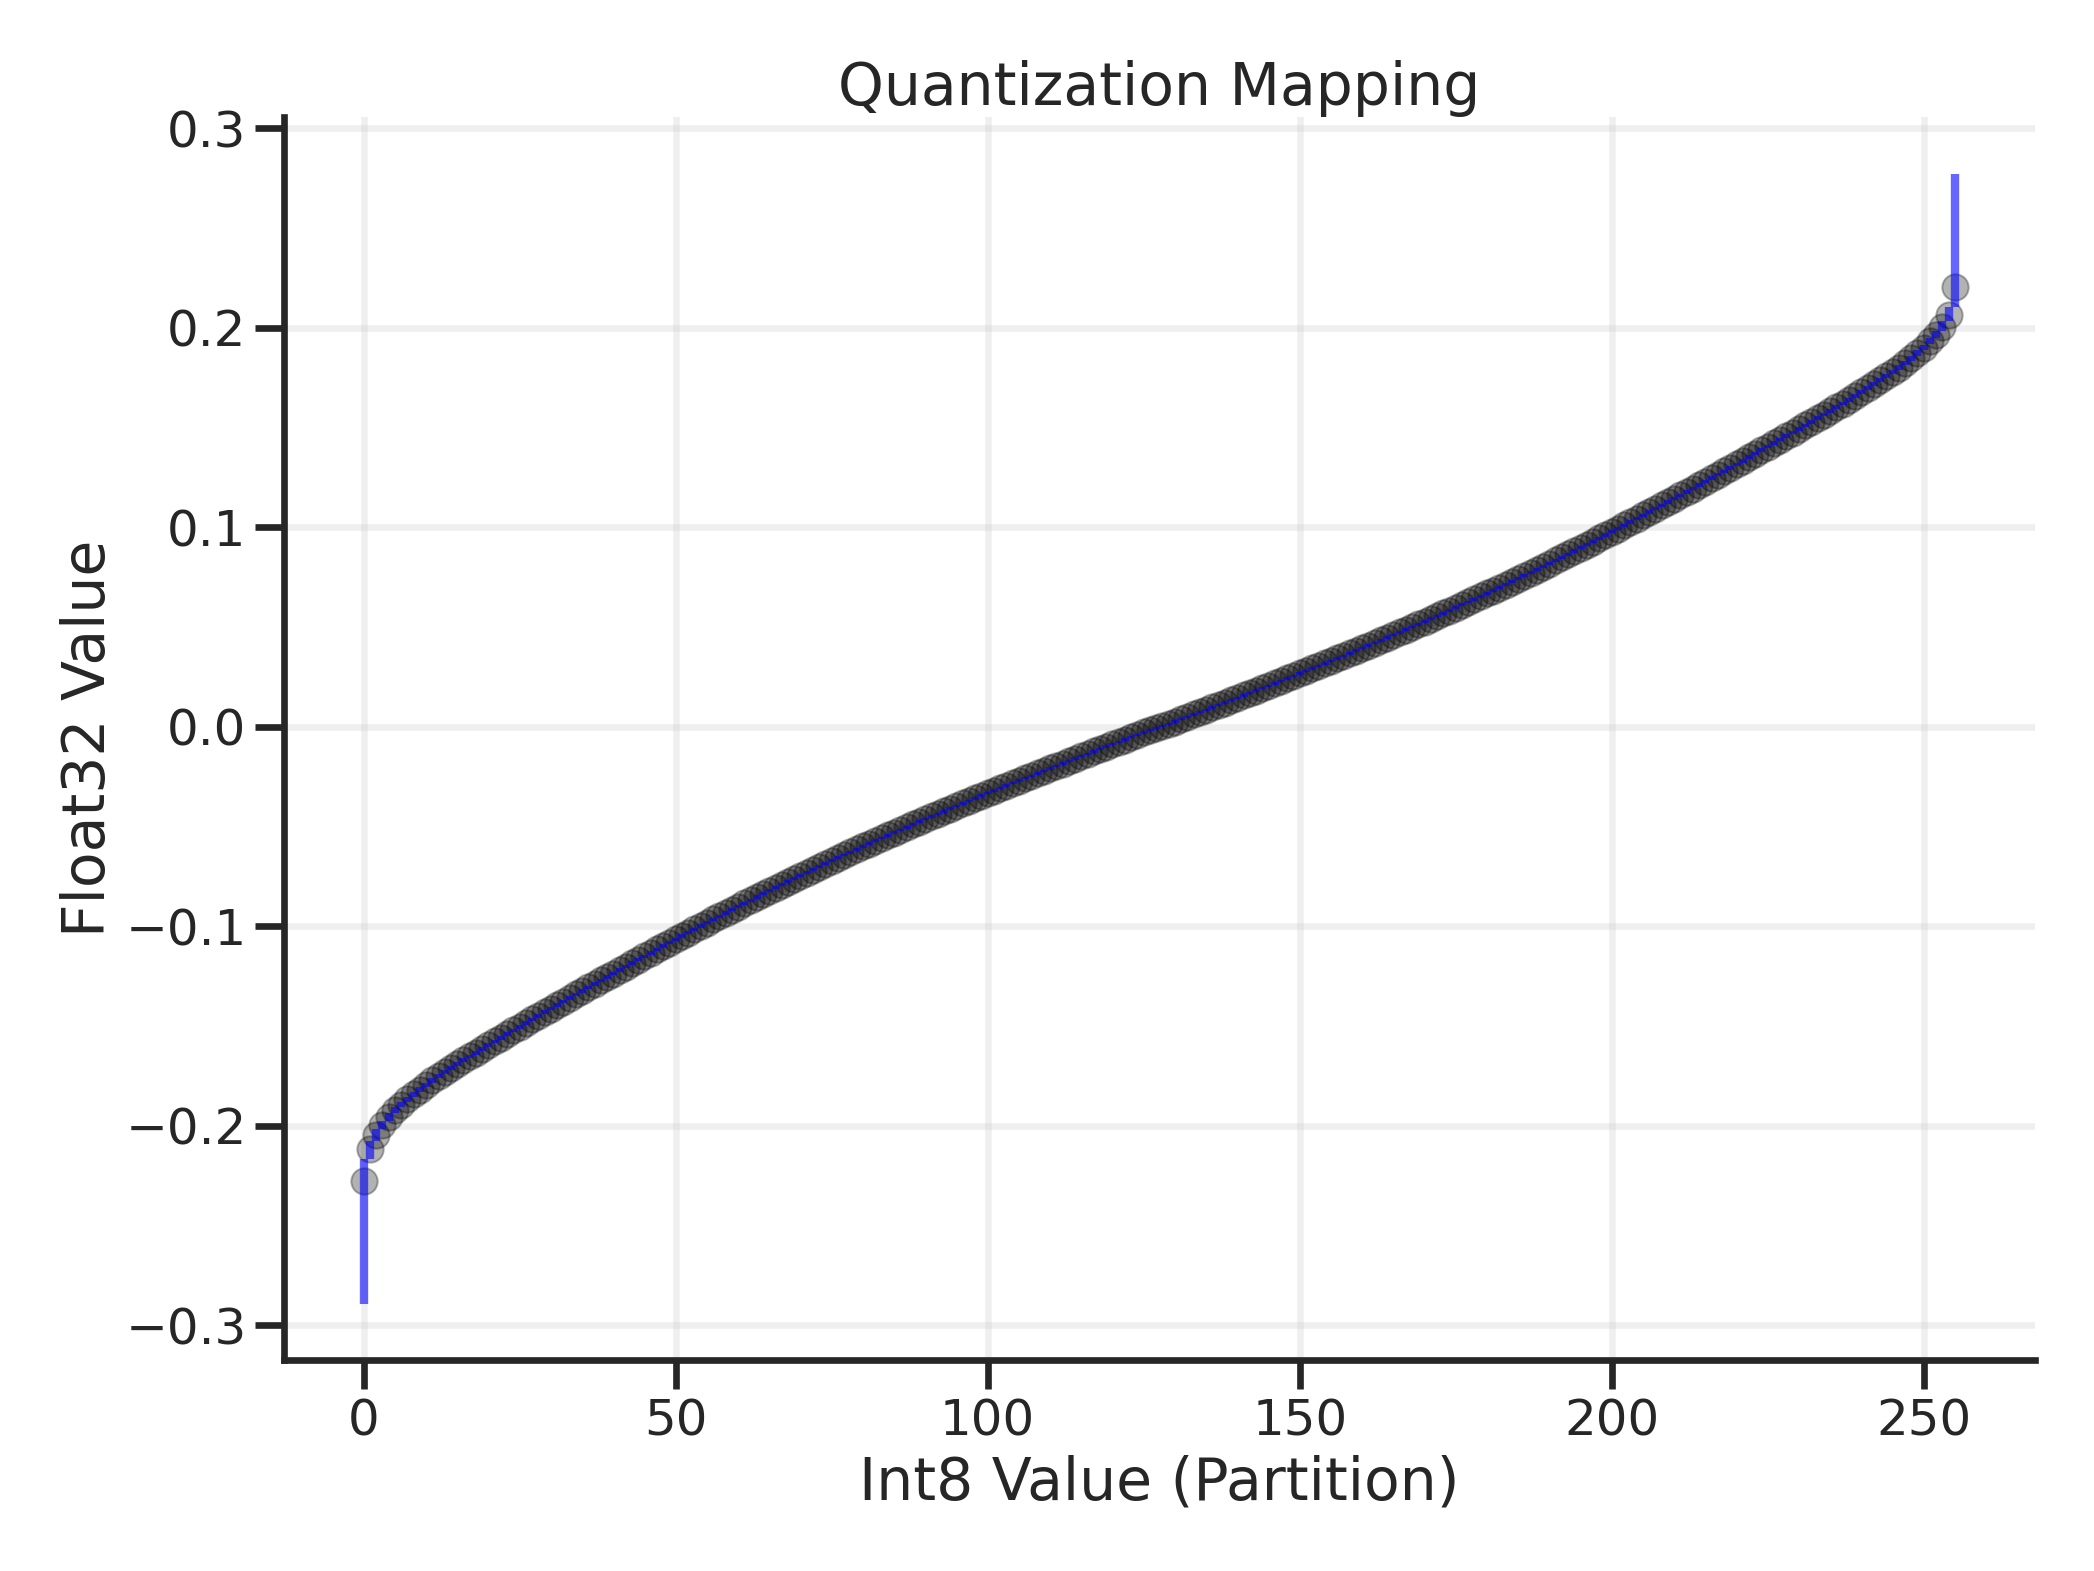
\includegraphics[width=0.49\widefigwidth]{bilder/plots/quantization_mapping_768.png}
      \vspace{-1cm}
      \caption{Mapped Float Quantization mapping for the sentence-transformers/all-mpnet-base-v2 model}
      \label{quantmapping768}
    \end{minipage}
  }
\end{figure}
\noindent The quantization mapping seen in \autoref{quantmapping768} of the embeddings from model \texttt{\seqsplit{sentence-transformers/all-mpnet-base-v2}} doesnt have a gap like the angle optimized model.\\\\
Varying k as seen in \autoref{kcomparison} doesn't create a big difference in accuracy.

\begin{figure}[h]
  \makebox[\textwidth][c]{%
    \begin{minipage}{0.49\widefigwidth}
      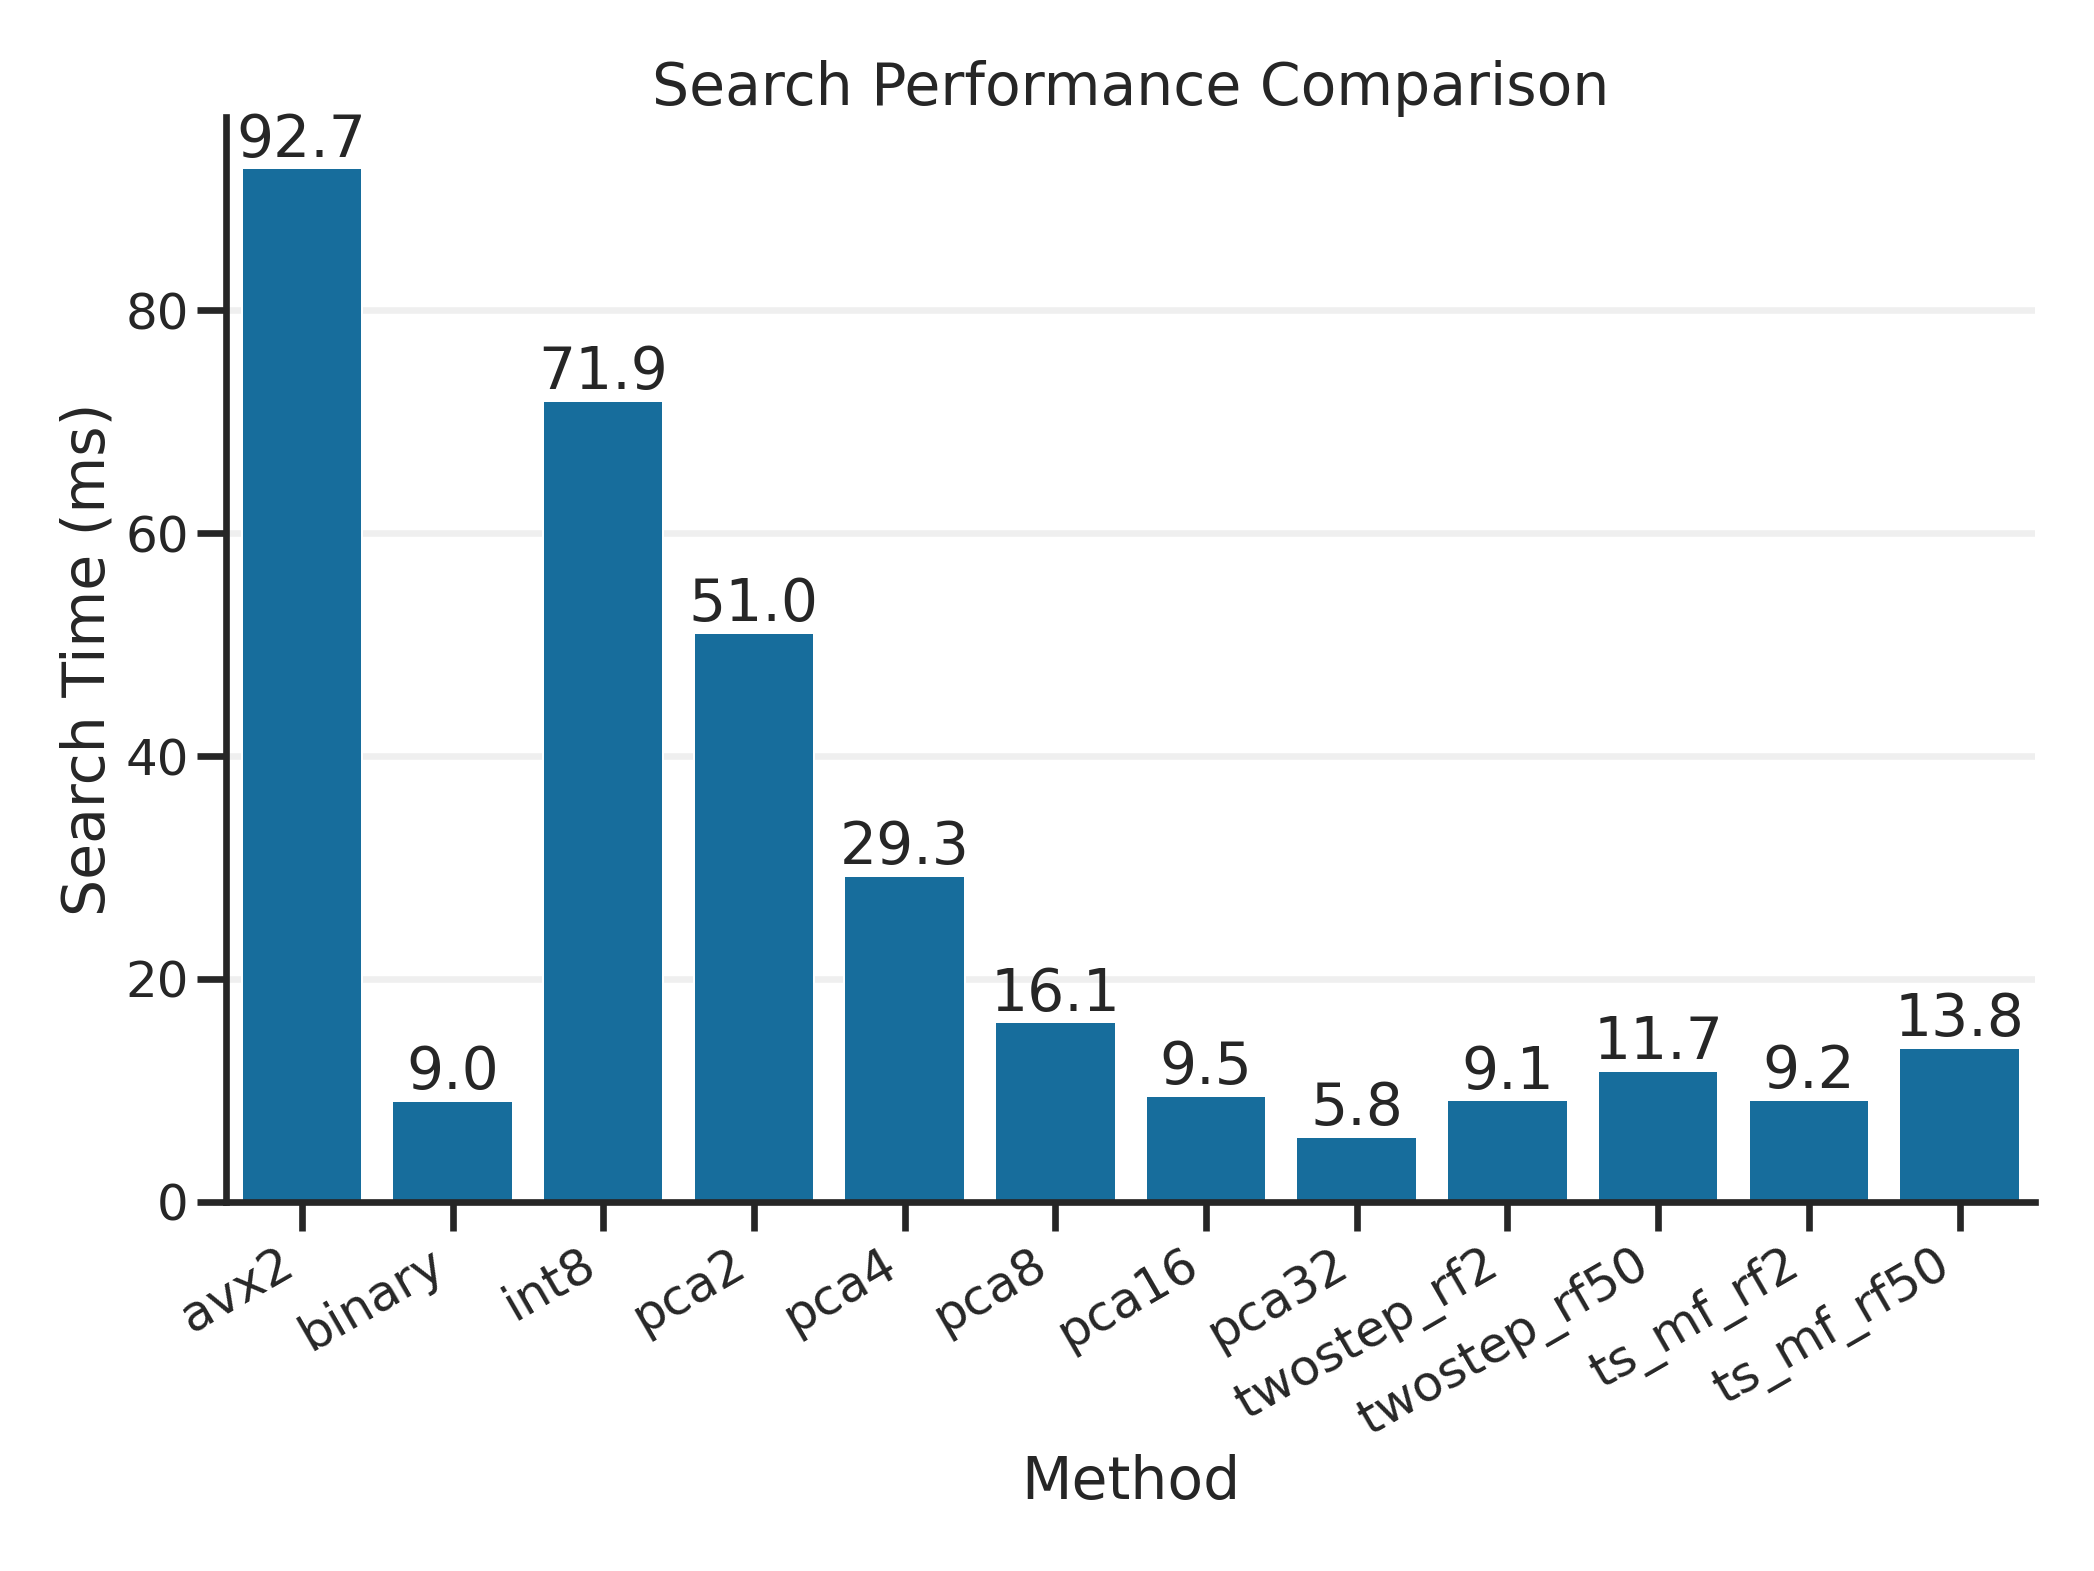
\includegraphics[width=0.49\widefigwidth]{bilder/plots/performance_comparison_dim768_k100_q.png}
      \vspace{-1cm}
      \caption{Search Speed vec\_dim=768 model: sentence-transformers/all-mpnet-base-v2}
    \end{minipage}
    %\hfill
    \begin{minipage}{0.49\widefigwidth}
      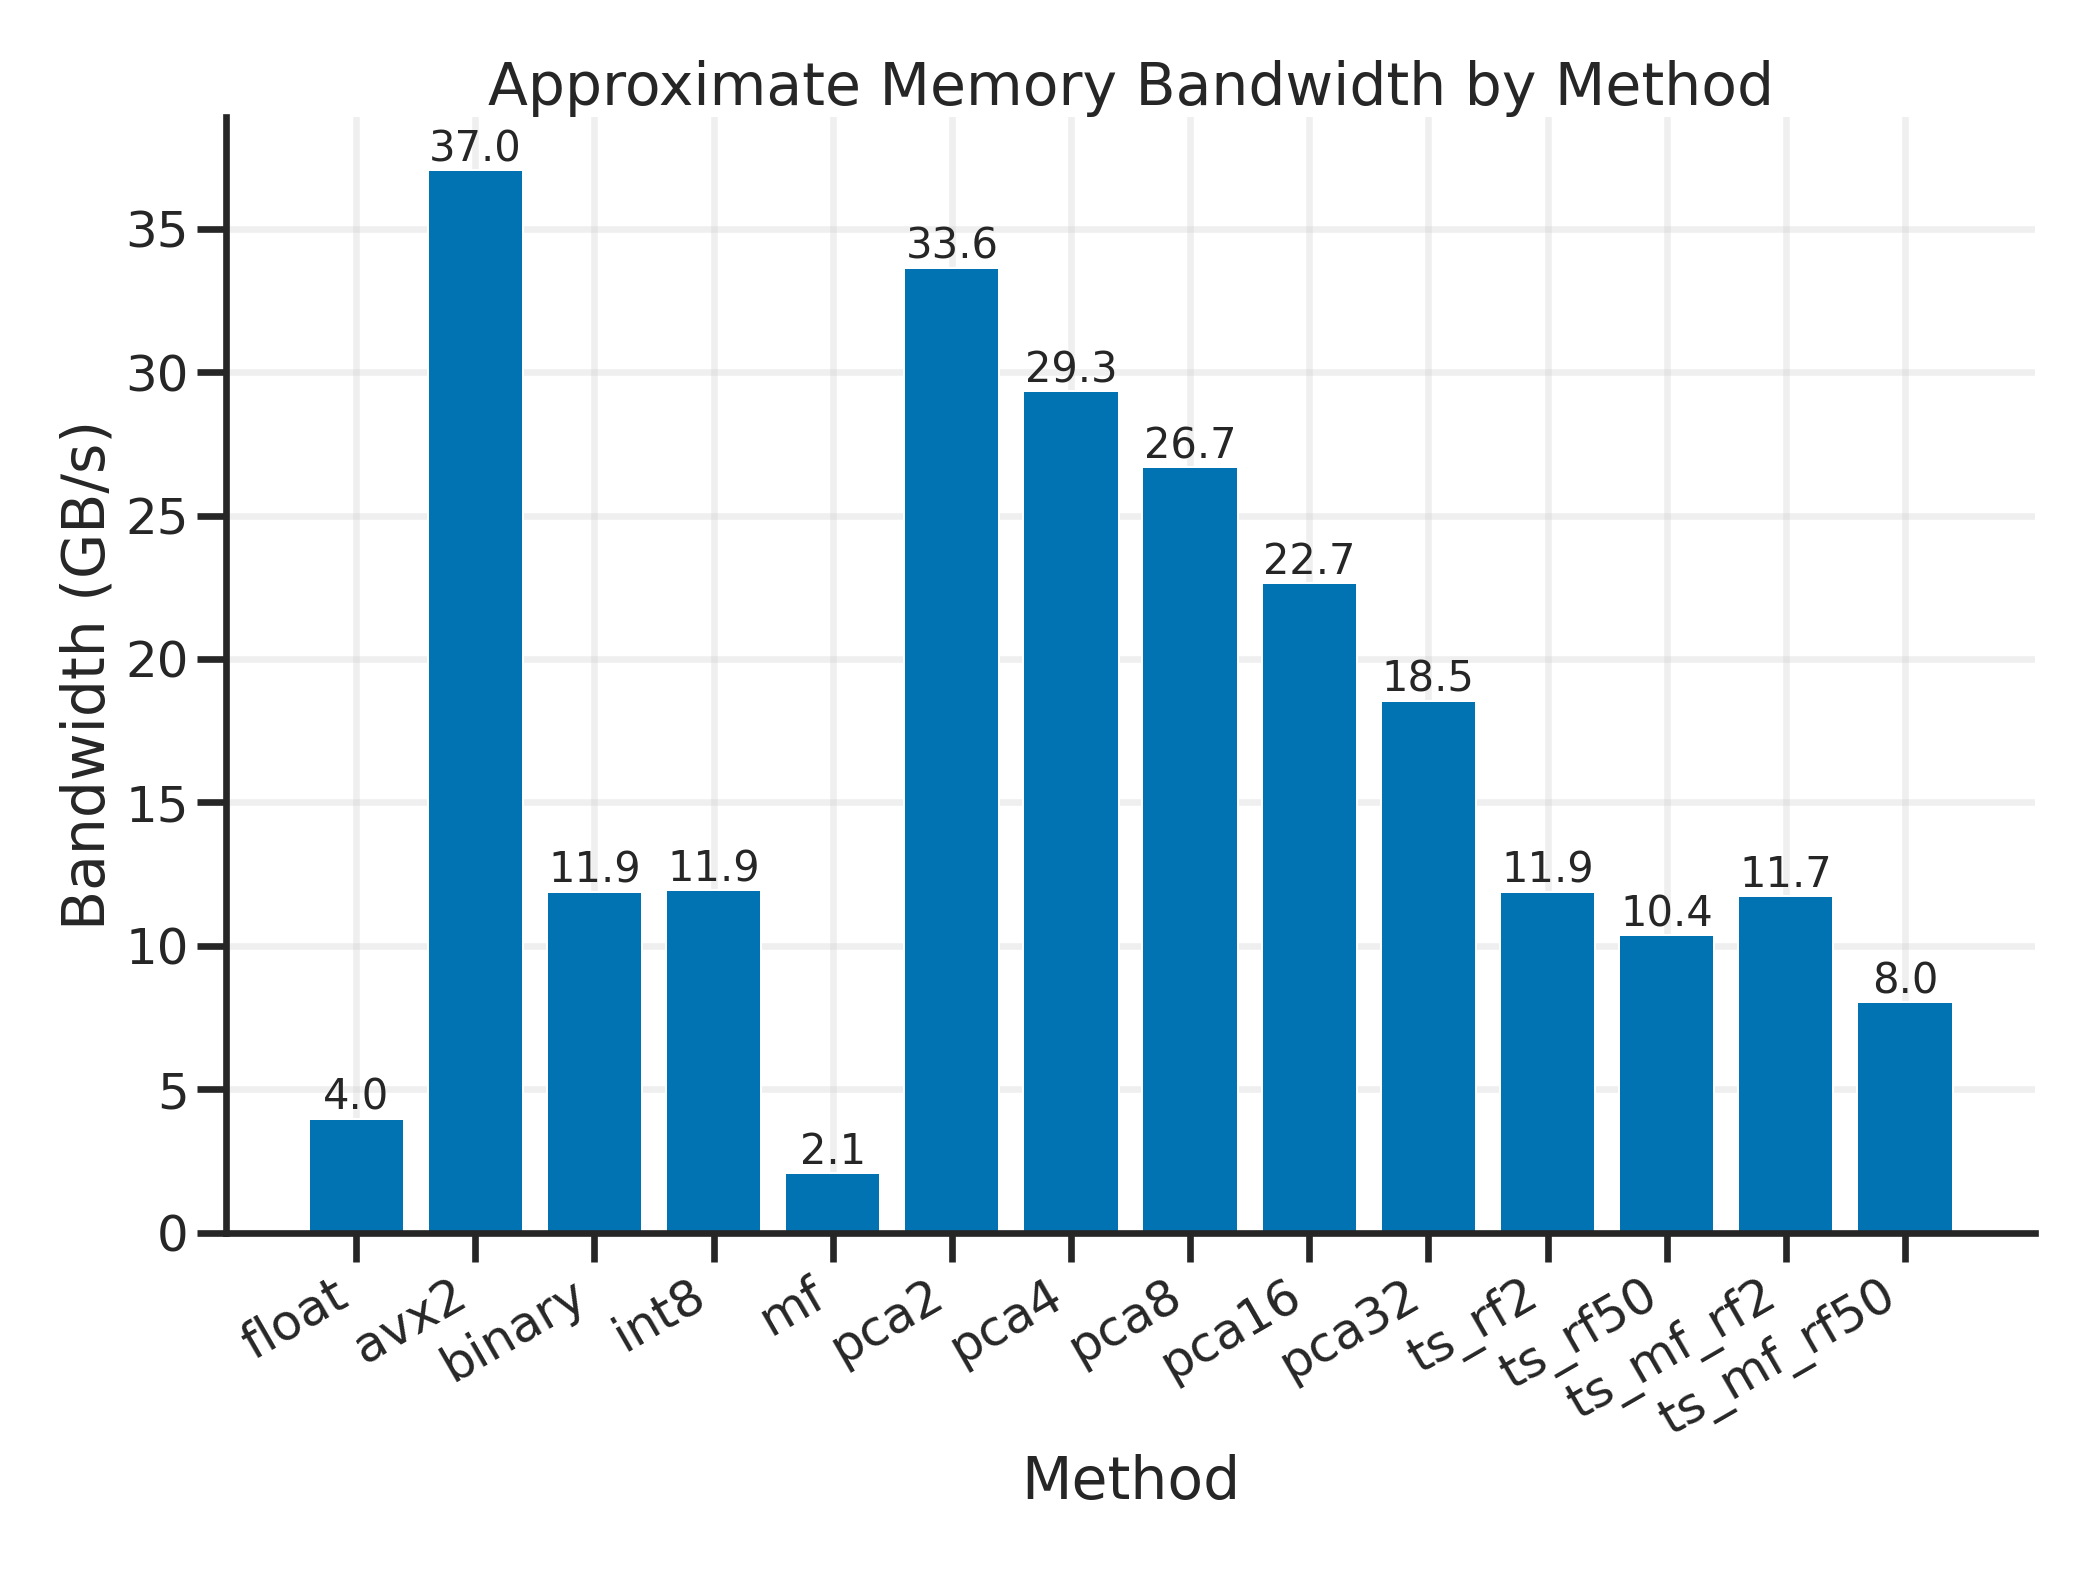
\includegraphics[width=0.49\widefigwidth]{bilder/plots/memory_bandwidth_benchmark_dim768_k100_q.png}
      \vspace{-1cm}
      \caption{Memory bandwidth vec\_dim=768 model: sentence-transformers/all-mpnet-base-v2}
      \label{memorybandwidth768}
    \end{minipage}
  }
\end{figure}
\noindent The memory bandwidth in \autoref{memorybandwidth768} when using the \texttt{\seqsplit{sentence-transformers/all-mpnet-base-v2}} model is even higher. The reason might be that higher striding distance is even better as this model creates embeddings of size 3072 bytes, so it has to use a striding distance of 12288 bytes as it's the first multiple that's divisible by 4096. Binary performs worse because it can't use the optimized unrolled loop as it only uses 3 avx2 vectors for 768 dimensions.

\begin{figure}[h]
  \makebox[\textwidth][c]{%
    \begin{minipage}{0.49\widefigwidth}
      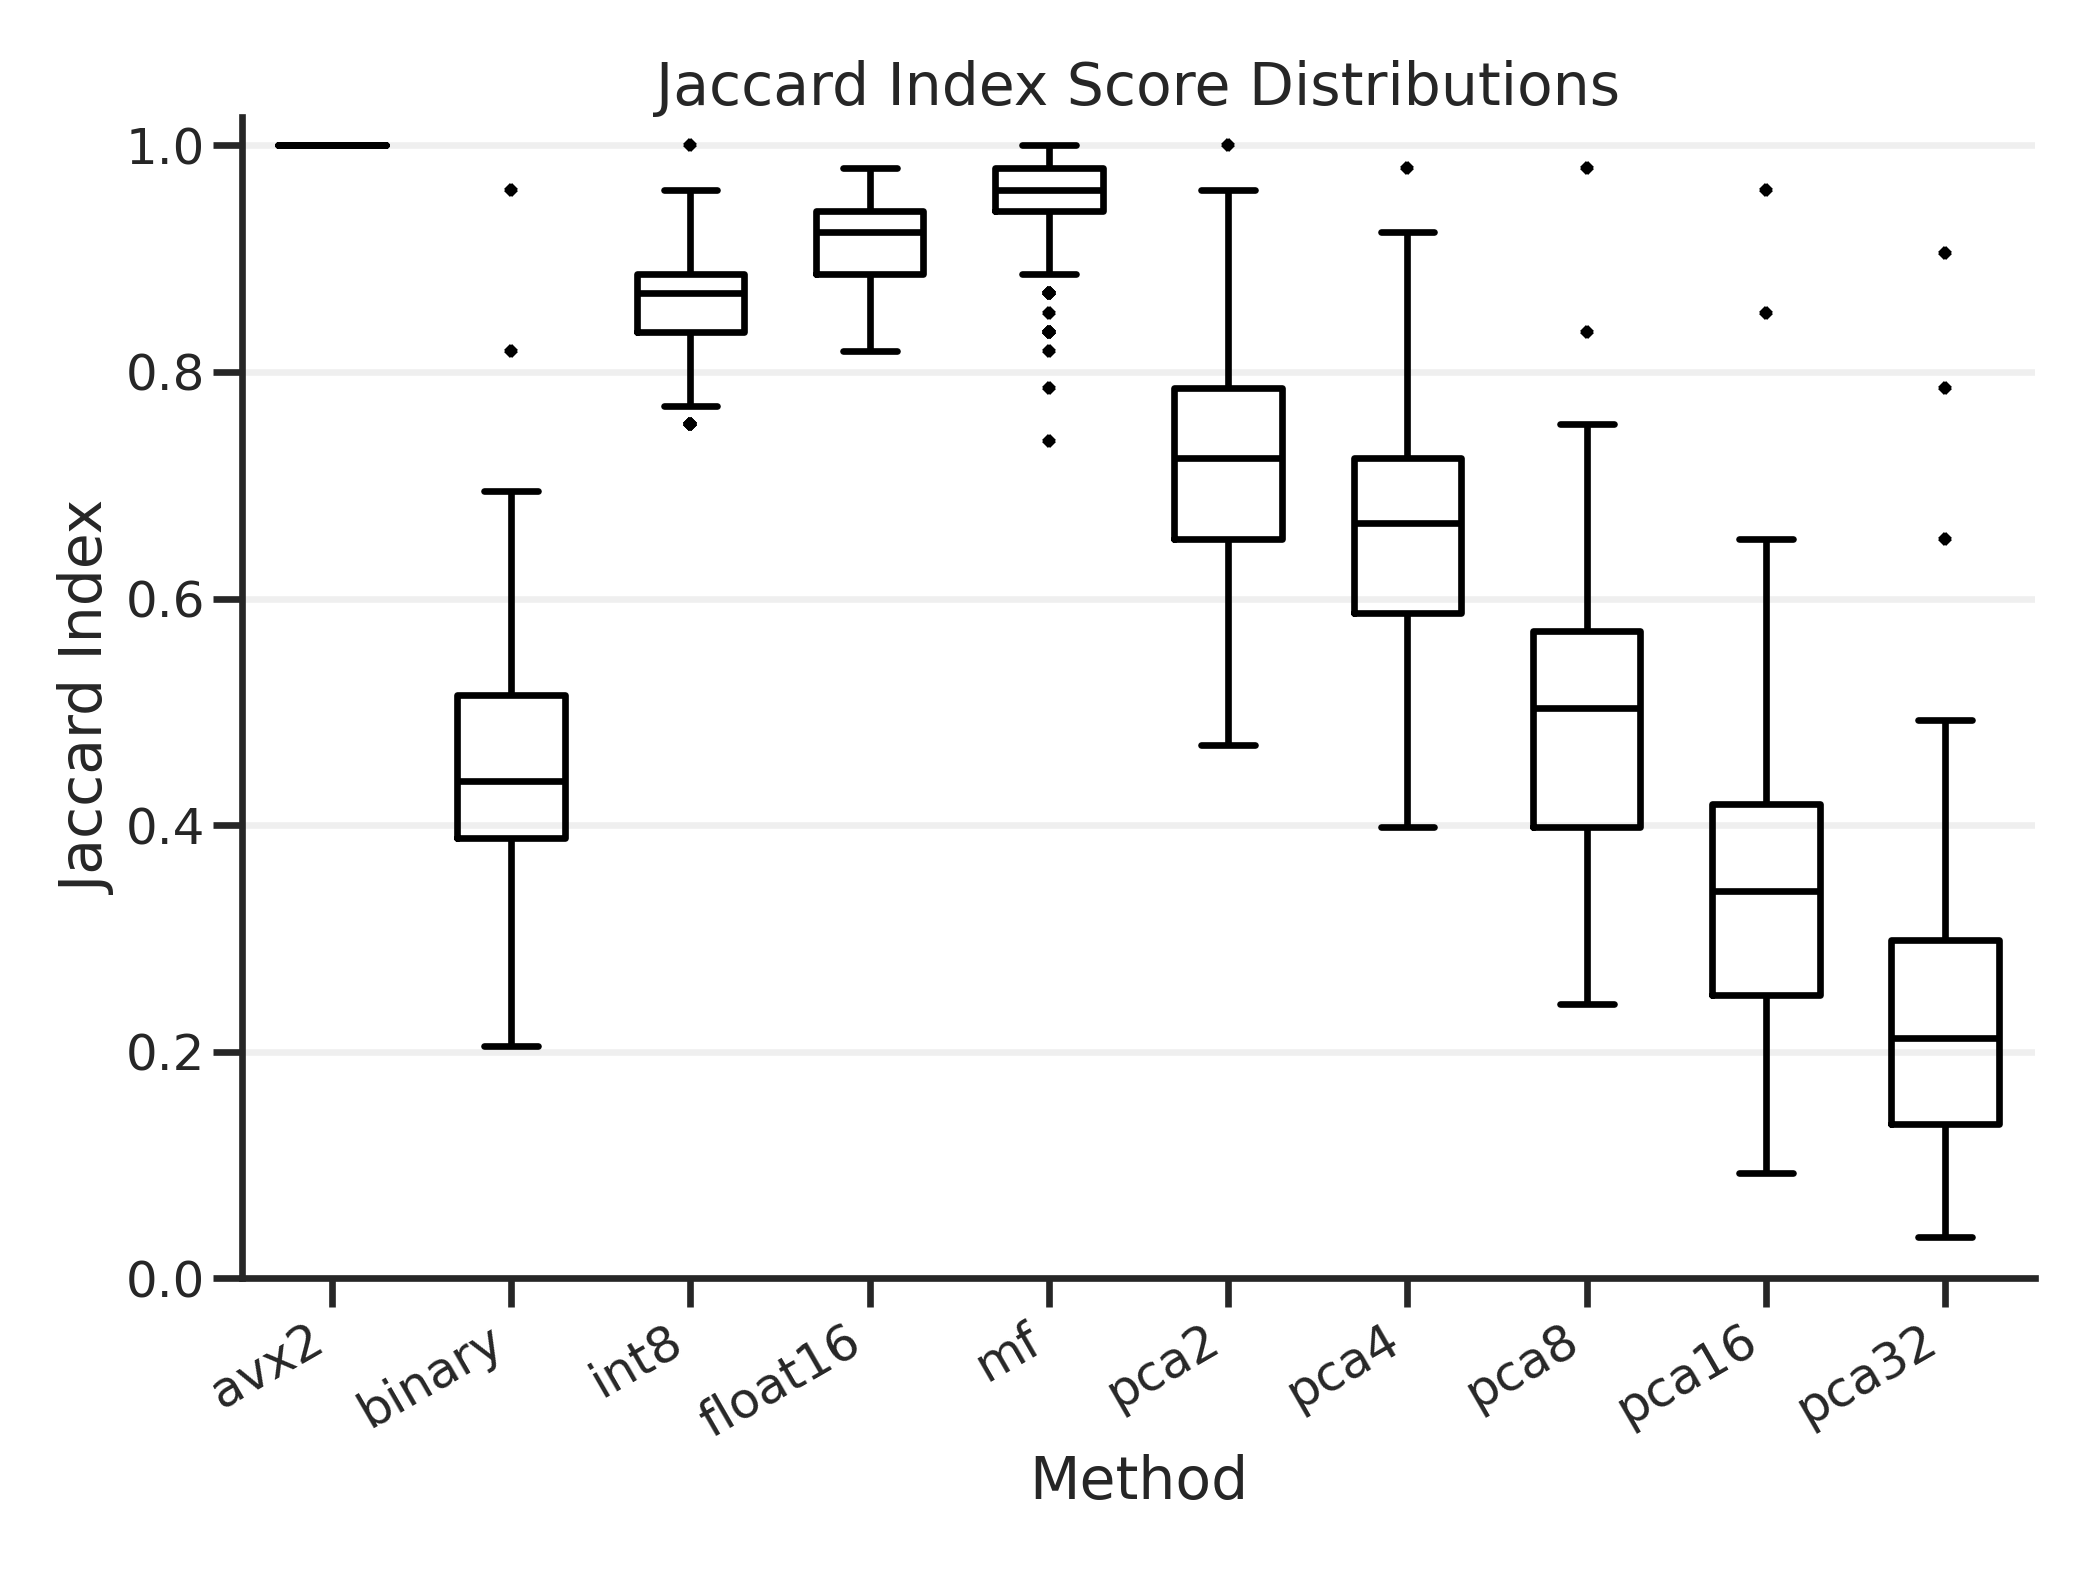
\includegraphics[width=0.49\widefigwidth]{bilder/plots/jaccard_boxplots_dim1024_k100_re.png}
      \vspace*{-1cm}
      \caption{Jaccard index of searchers with randomly generated queries}
      \label{boxjaccardsearchersone-re}
    \end{minipage}
    %\hfill
    \begin{minipage}{0.49\widefigwidth}
      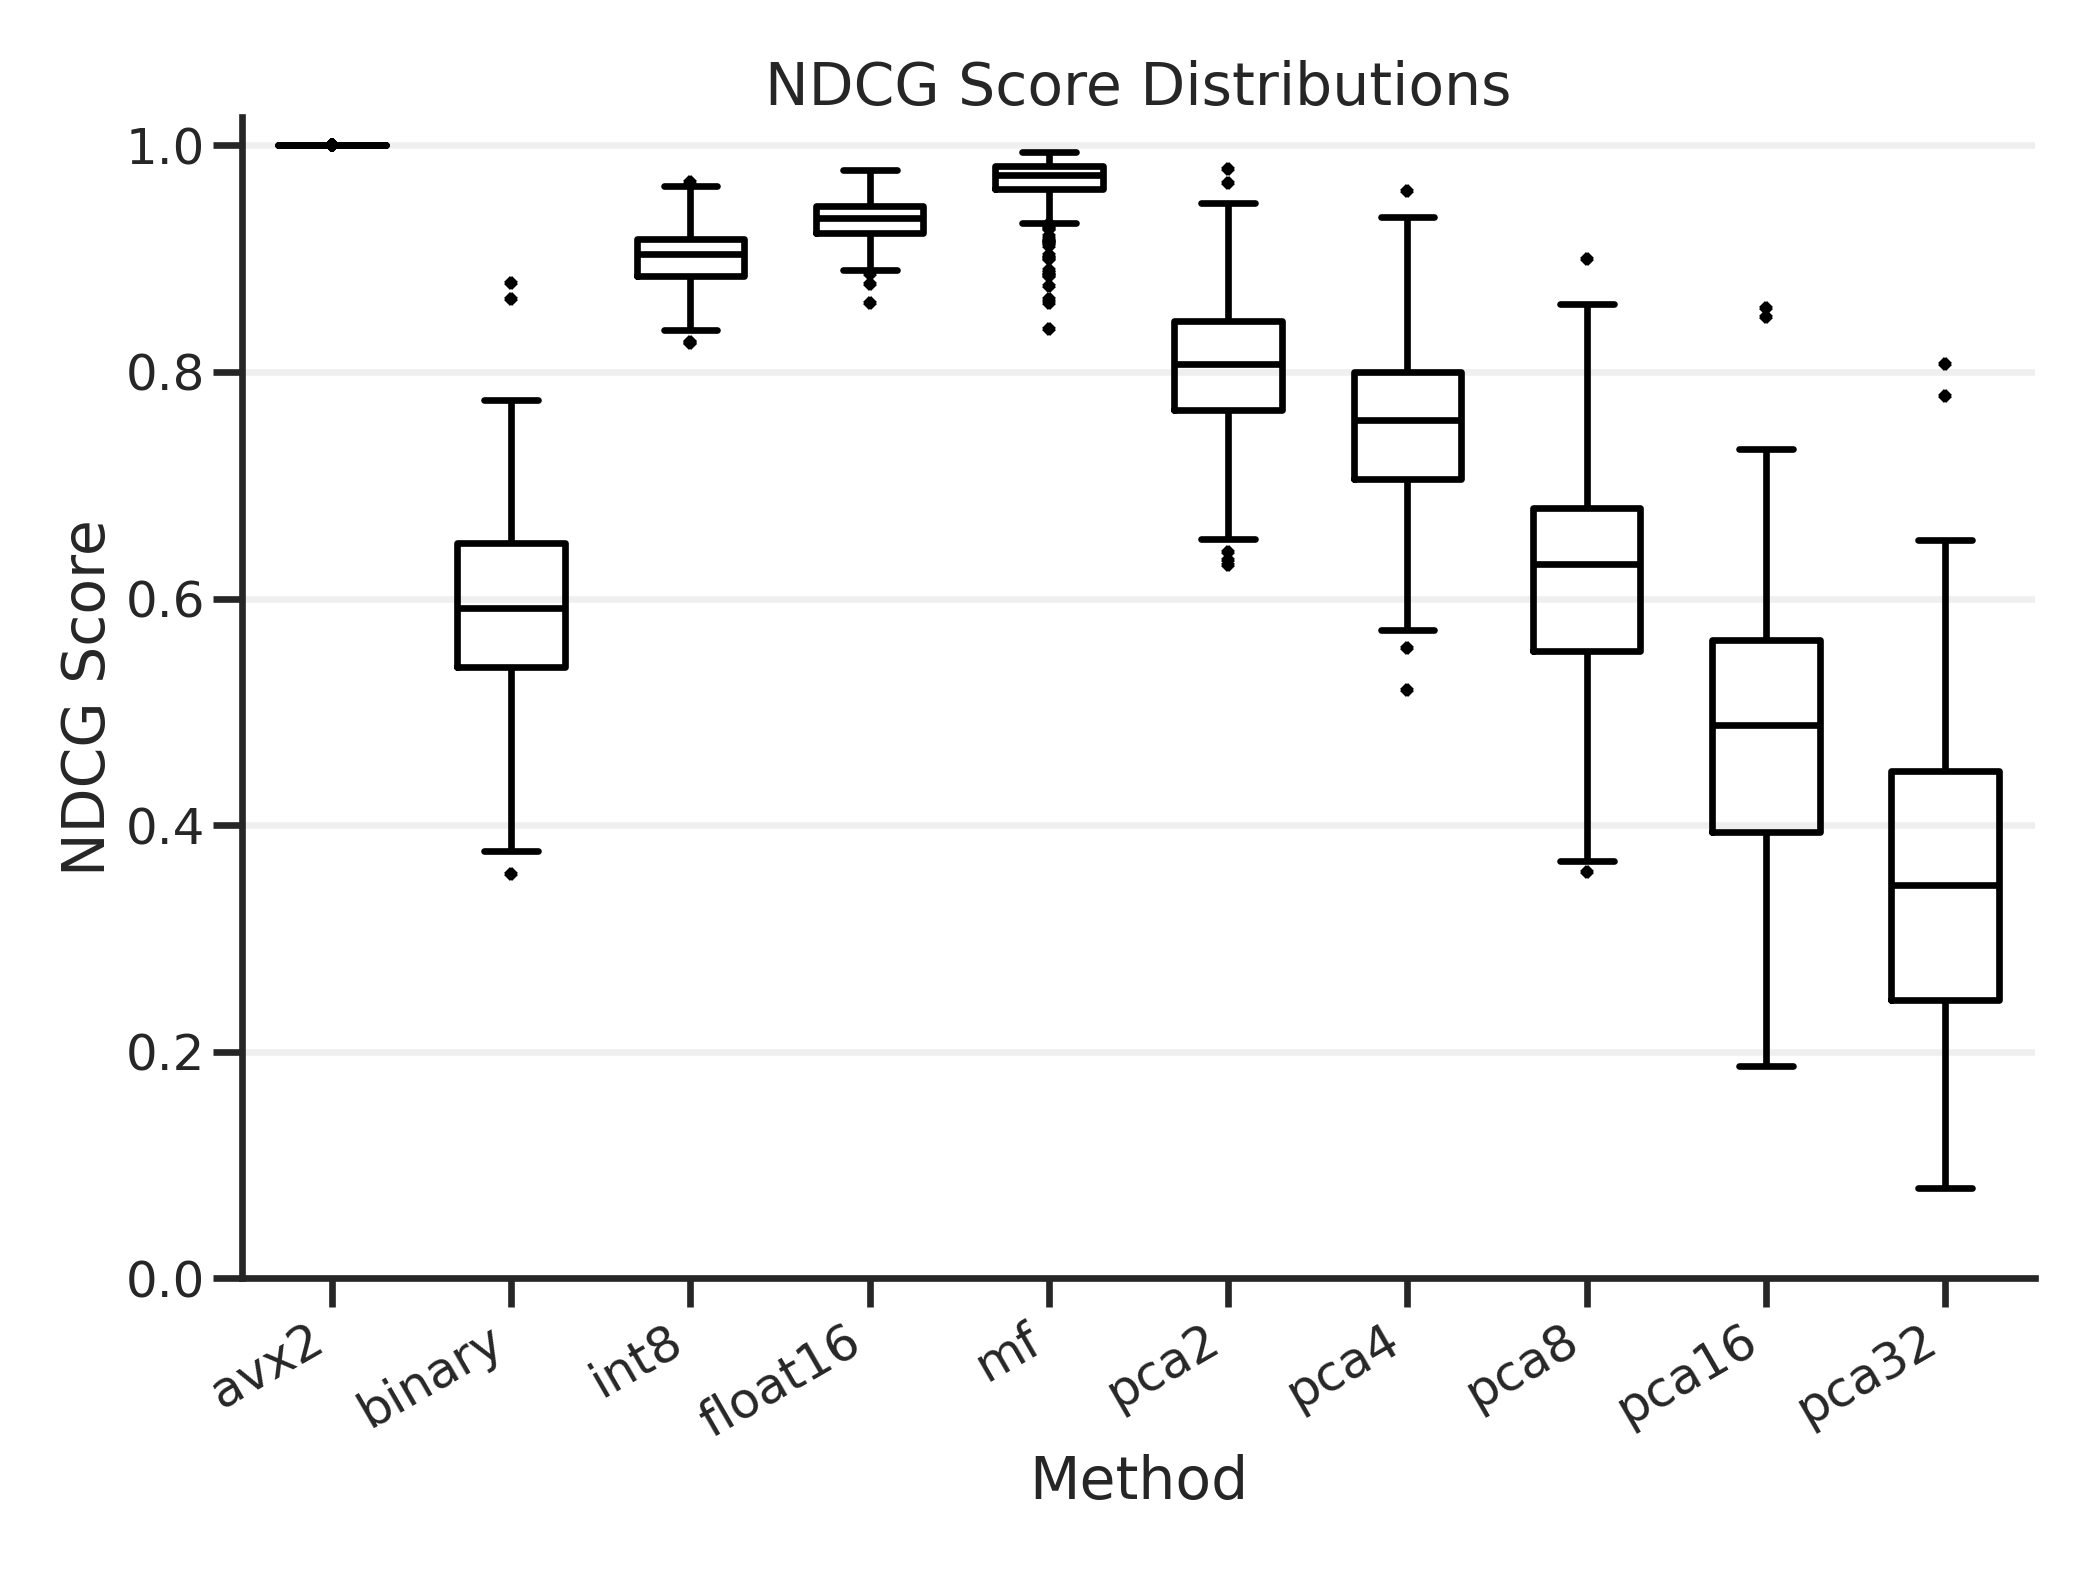
\includegraphics[width=0.49\widefigwidth]{bilder/plots/ndcg_boxplots_dim1024_k100_re.png}
      \vspace*{-1cm}
      \caption{NDCG score of searchers with randomly generated queries}
      \label{boxndcgsearchersone-re}
    \end{minipage}
  }
\end{figure}
\begin{figure}[h]
  \makebox[\textwidth][c]{%
    \begin{minipage}{0.49\widefigwidth}
      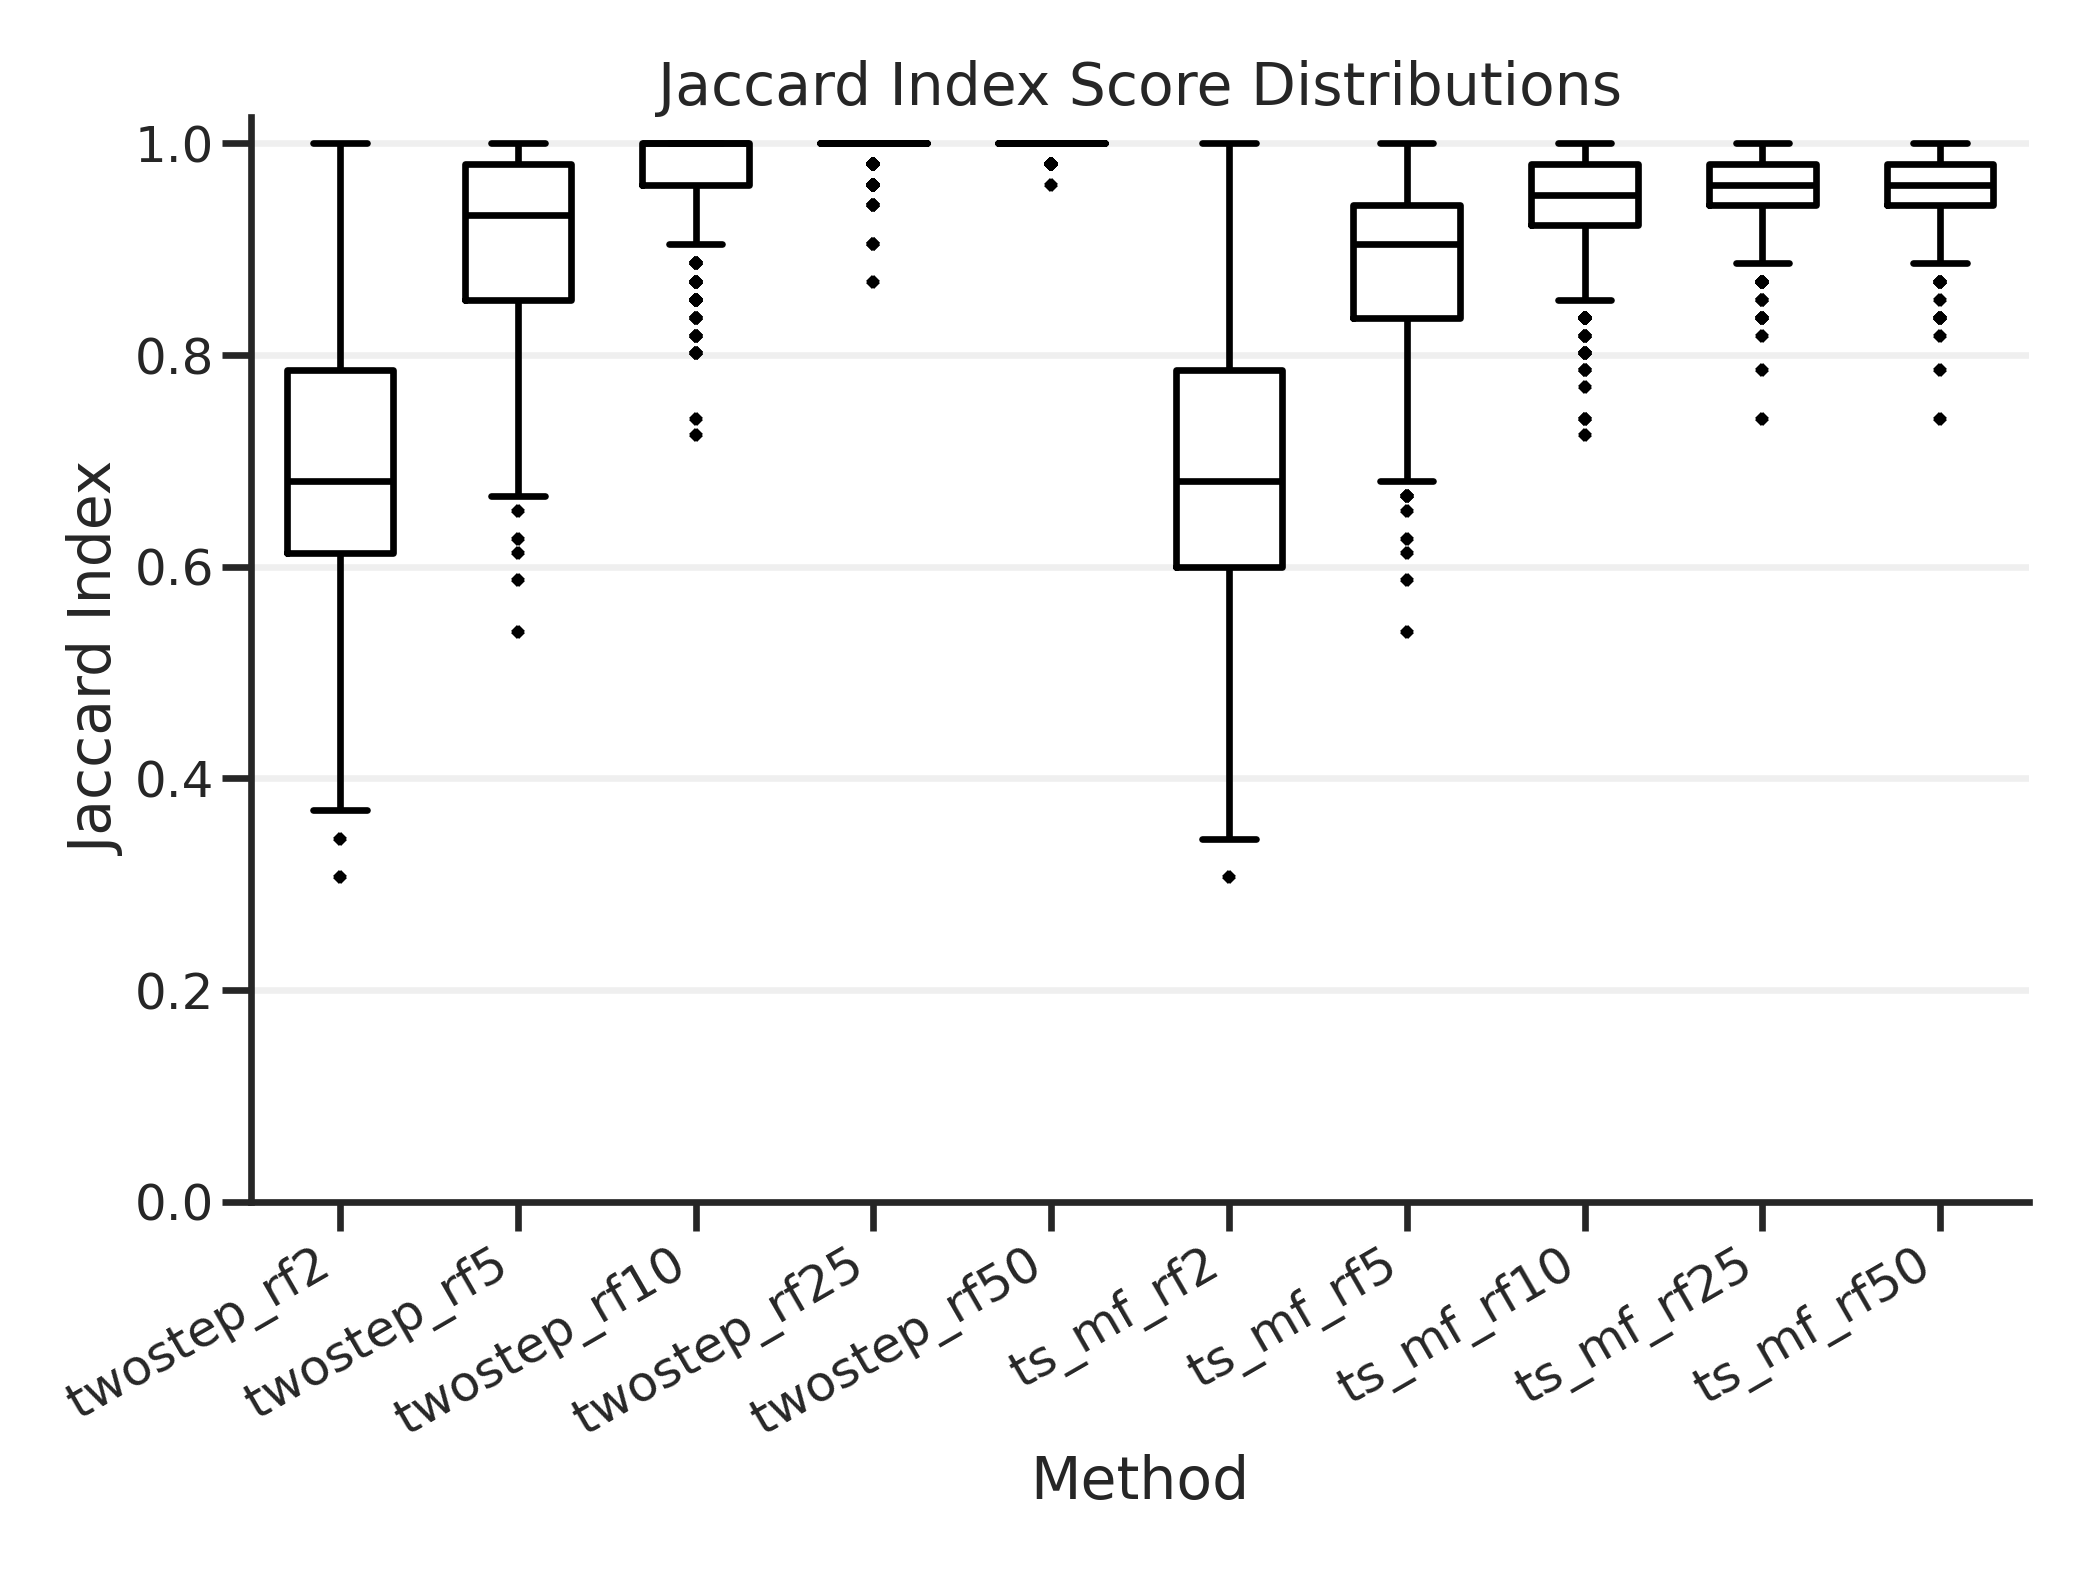
\includegraphics[width=0.49\widefigwidth]{bilder/plots/jaccard_boxplots_dim1024_k100_re_twostep.png}
      \vspace*{-1cm}
      \caption{Jaccard index of two-step searchers with randomly generated queries}
      \label{boxjaccardsearcherstwo-re}
    \end{minipage}
    %\hfill
    \begin{minipage}{0.49\widefigwidth}
      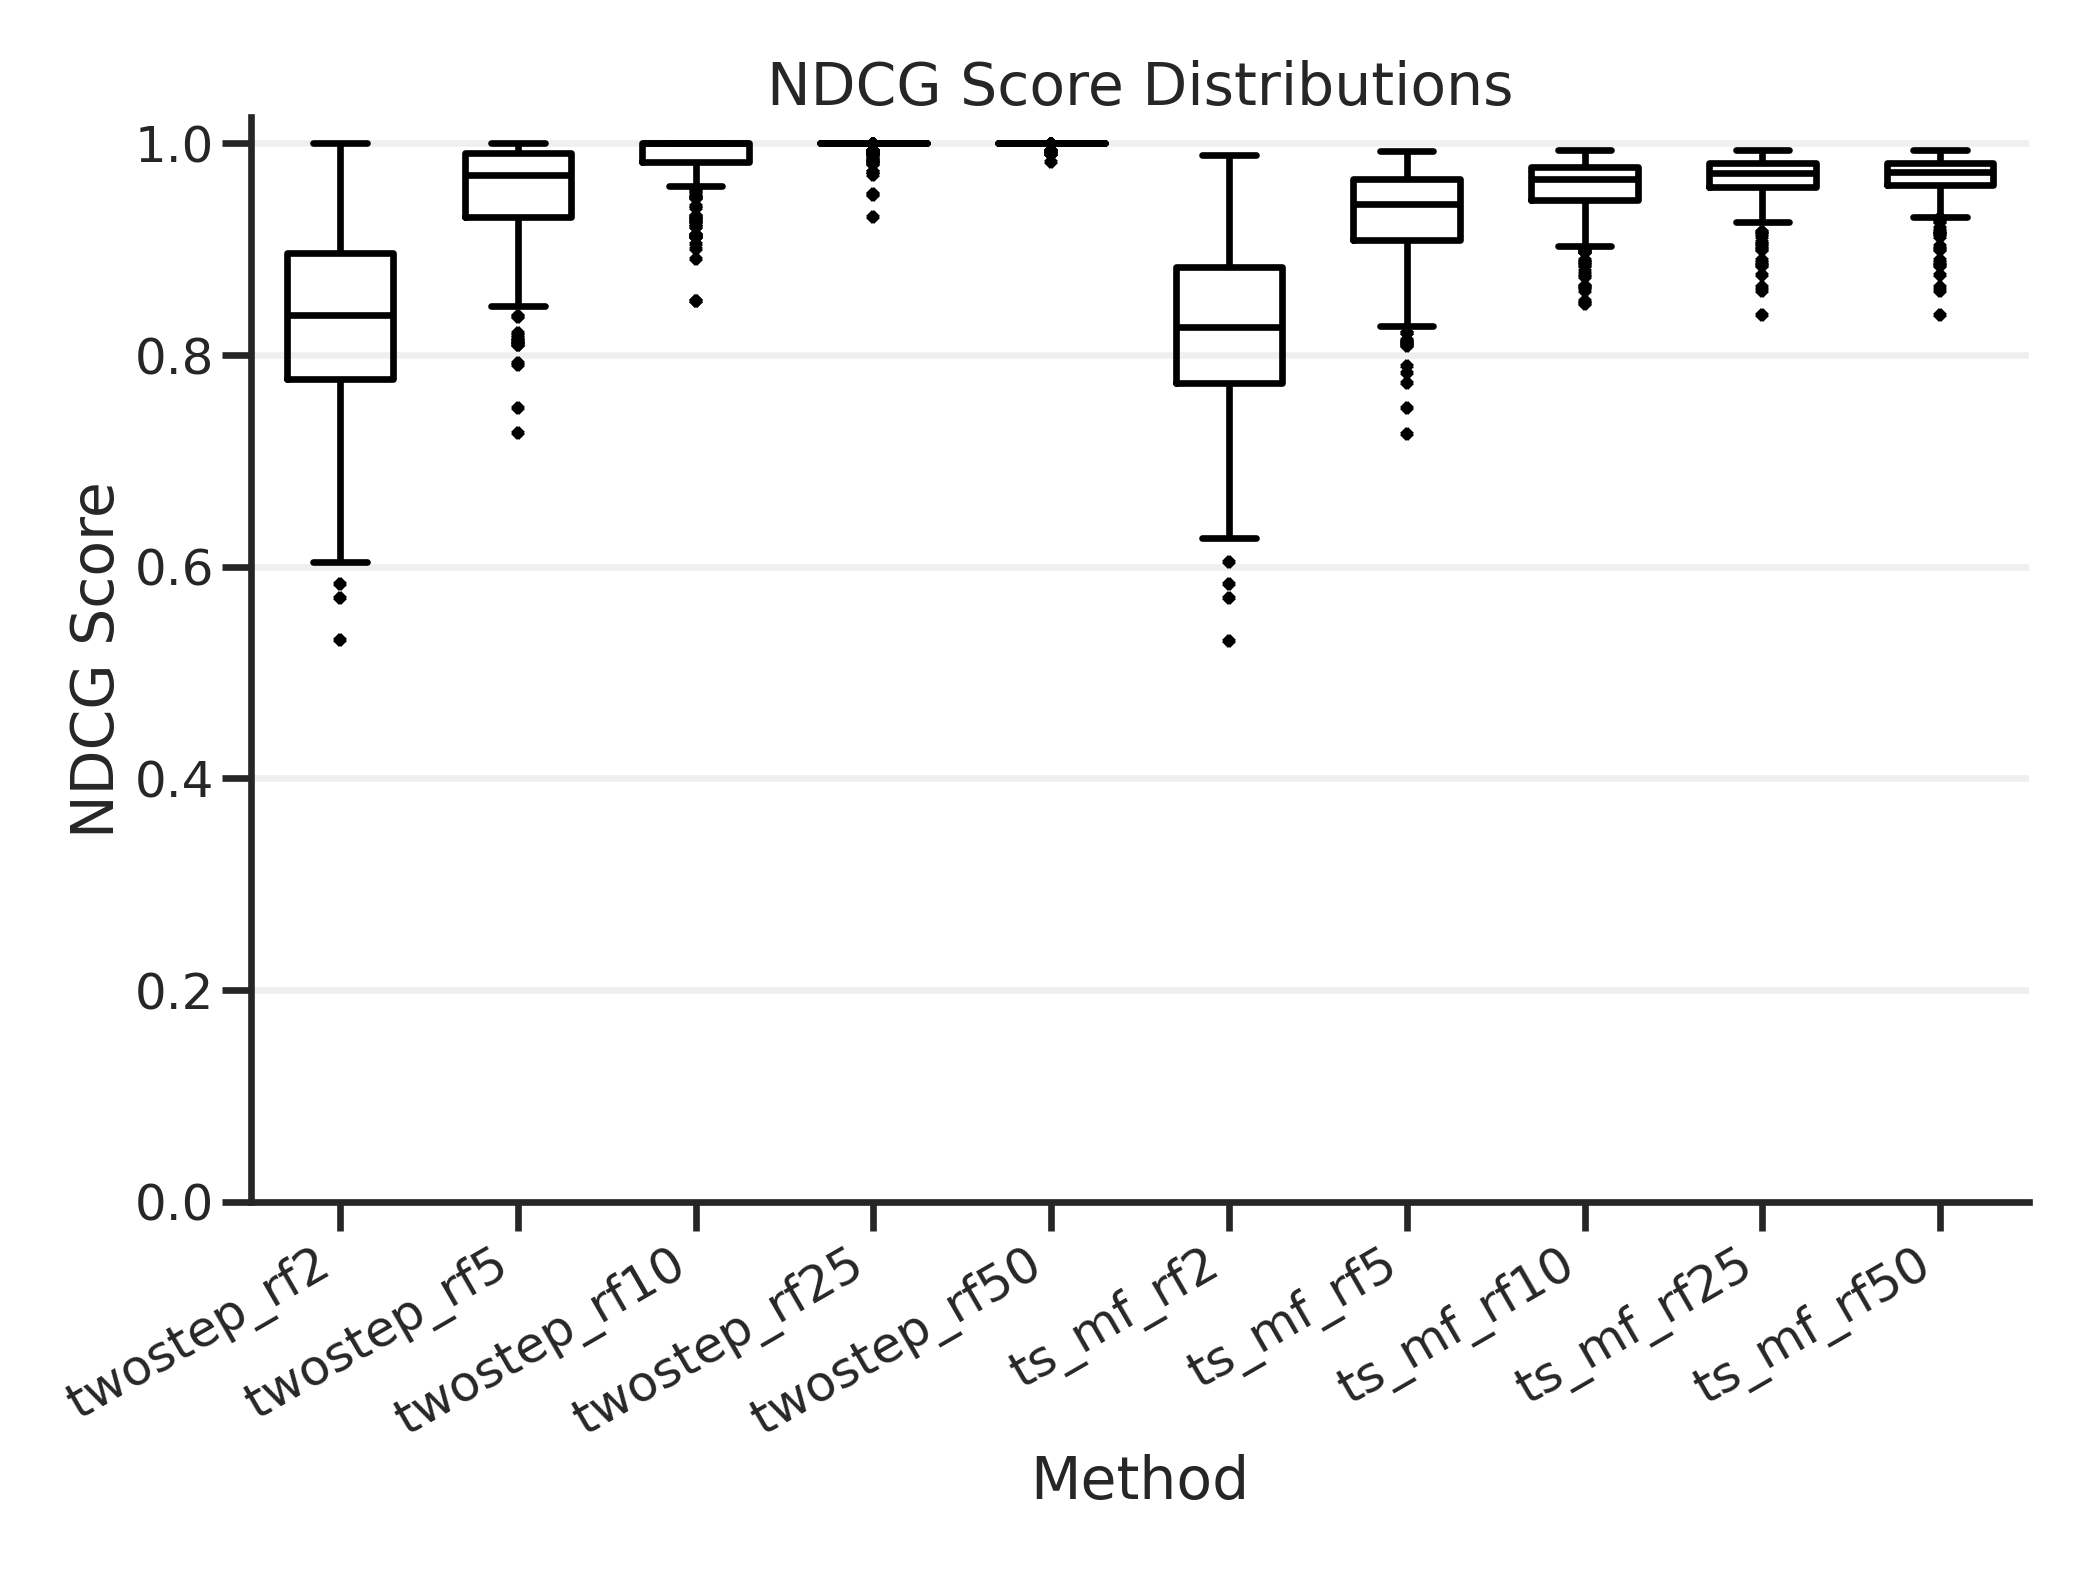
\includegraphics[width=0.49\widefigwidth]{bilder/plots/ndcg_boxplots_dim1024_k100_re_twostep.png}
      \vspace*{-1cm}
      \caption{NDCG score of two-step searchers with randomly generated queries}
      \label{boxndcgsearcherstwo-re}
    \end{minipage}
  }
\end{figure}
Looking at \autoref{boxjaccardsearchersone-re} \ref{boxndcgsearchersone-re} \ref{boxjaccardsearcherstwo-re} \ref{boxndcgsearcherstwo-re}: The searchers perform worse in accuracy across the board. But this isn't a drawback as this is not a realistic use case for embedding search.

\begin{table}[h]
  \centering
  \begin{tabular}{lccccccc}
    \hline
    Method       & Mean (ms) & Std Time & NDCG  & Jaccard & Overlap & M (GB) & BW (GB/s) \\
    \hline
    float        & 1105.232  & 0.948    & 1.000 & 1.000   & 100.000 & 4.578  & 4.142     \\
    avx2         & 135.972   & 1.105    & 1.000 & 1.000   & 100.000 & 4.578  & 33.666    \\
    binary       & 6.662     & 0.048    & 0.589 & 0.451   & 61.496  & 0.143  & 21.474    \\
    int8         & 95.215    & 0.055    & 0.901 & 0.867   & 92.836  & 1.144  & 12.019    \\
    float16      & 185.023   & 6.713    & 0.934 & 0.914   & 95.500  & 2.289  & 12.370    \\
    mf           & 540.883   & 0.325    & 0.966 & 0.956   & 97.692  & 1.144  & 2.116     \\
    pca2         & 71.421    & 0.607    & 0.803 & 0.724   & 83.700  & 2.291  & 32.047    \\
    pca4         & 38.725    & 0.314    & 0.750 & 0.653   & 78.544  & 1.145  & 29.552    \\
    pca8         & 22.146    & 0.217    & 0.616 & 0.489   & 64.820  & 0.573  & 25.838    \\
    pca16        & 12.469    & 0.201    & 0.482 & 0.346   & 50.140  & 0.286  & 22.944    \\
    pca32        & 7.566     & 0.129    & 0.351 & 0.228   & 35.720  & 0.143  & 18.908    \\
    twos\_rf2    & 6.583     & 0.065    & 0.830 & 0.689   & 80.772  & 4.721  & 21.846    \\
    twos\_rf5    & 6.727     & 0.063    & 0.952 & 0.904   & 94.660  & 4.721  & 21.550    \\
    twos\_rf10   & 7.006     & 0.067    & 0.985 & 0.969   & 98.344  & 4.721  & 20.963    \\
    twos\_rf25   & 7.952     & 0.089    & 0.998 & 0.995   & 99.748  & 4.721  & 19.188    \\
    twos\_rf50   & 9.486     & 0.124    & 1.000 & 0.999   & 99.948  & 4.721  & 17.091    \\
    ts\_mf\_rf2  & 6.600     & 0.054    & 0.821 & 0.684   & 80.452  & 1.287  & 21.702    \\
    ts\_mf\_rf5  & 6.930     & 0.053    & 0.930 & 0.880   & 93.384  & 1.287  & 20.711    \\
    ts\_mf\_rf10 & 7.476     & 0.062    & 0.956 & 0.934   & 96.516  & 1.287  & 19.262    \\
    ts\_mf\_rf25 & 9.131     & 0.086    & 0.965 & 0.953   & 97.548  & 1.287  & 15.927    \\
    ts\_mf\_rf50 & 11.820    & 0.136    & 0.966 & 0.955   & 97.668  & 1.287  & 12.506    \\
    \hline
  \end{tabular}
  \caption{Comparison of methods for mixedbread-ai/mxbai-embed-large-v1}
  \label{tab:method-comparison-1024}
\end{table}

\begin{table}[h]
  \centering
  \begin{tabular}{lccccccc}
    \hline
    Method       & Mean (ms) & Std Time & NDCG  & Jaccard & Overlap & M (GB) & BW (GB/s) \\
    \hline
    float        & 862.587   & 0.625    & 1.000 & 1.000   & 100.000 & 3.433  & 3.980     \\
    avx2         & 91.731    & 1.469    & 1.000 & 1.000   & 100.000 & 3.433  & 37.427    \\
    binary       & 9.022     & 0.063    & 0.605 & 0.475   & 63.664  & 0.107  & 11.891    \\
    int8         & 72.253    & 0.094    & 0.930 & 0.910   & 95.248  & 0.858  & 11.879    \\
    float16      & 142.844   & 18.197   & 0.967 & 0.959   & 97.880  & 1.717  & 12.017    \\
    mf           & 408.601   & 0.357    & 0.992 & 0.989   & 99.468  & 0.858  & 2.101     \\
    pca2         & 51.656    & 0.481    & 0.901 & 0.864   & 92.624  & 1.718  & 33.231    \\
    pca4         & 29.478    & 0.331    & 0.820 & 0.754   & 85.648  & 0.859  & 29.117    \\
    pca8         & 16.082    & 0.156    & 0.626 & 0.505   & 66.076  & 0.429  & 26.685    \\
    pca16        & 9.487     & 0.141    & 0.441 & 0.309   & 45.680  & 0.215  & 22.618    \\
    pca32        & 5.767     & 0.112    & 0.285 & 0.174   & 28.260  & 0.107  & 18.602    \\
    twos\_rf2    & 9.076     & 0.031    & 0.848 & 0.717   & 82.772  & 3.541  & 11.884    \\
    twos\_rf5    & 9.241     & 0.031    & 0.962 & 0.924   & 95.828  & 3.541  & 11.764    \\
    twos\_rf10   & 9.521     & 0.034    & 0.991 & 0.981   & 99.008  & 3.541  & 11.569    \\
    twos\_rf25   & 10.404    & 0.060    & 0.999 & 0.998   & 99.900  & 3.541  & 11.000    \\
    twos\_rf50   & 11.816    & 0.101    & 1.000 & 1.000   & 99.976  & 3.541  & 10.291    \\
    ts\_mf\_rf2  & 9.157     & 0.065    & 0.847 & 0.717   & 82.760  & 0.966  & 11.732    \\
    ts\_mf\_rf5  & 9.465     & 0.024    & 0.959 & 0.921   & 95.684  & 0.966  & 11.373    \\
    ts\_mf\_rf10 & 9.965     & 0.034    & 0.985 & 0.974   & 98.632  & 0.966  & 10.839    \\
    ts\_mf\_rf25 & 11.479    & 0.063    & 0.991 & 0.988   & 99.384  & 0.966  & 9.502     \\
    ts\_mf\_rf50 & 13.903    & 0.113    & 0.992 & 0.989   & 99.444  & 0.966  & 7.974     \\
    \hline
  \end{tabular}
  \caption{Comparison of methods for sentence-transformers/all-mpnet-base-v2}
  \label{tab:method-comparison-768}
\end{table}